\begin{figure}
  \caption{Dependence of Social Learning ($\langle s \rangle$) on environmental
  variability $u$ for several values of low payoff $\pisub{low}$, number of
  behaviors $B$, and steps per round, $M = 0.5B,~B,~2B$. Average over 70 trials
at the final time step \mt{full 100 imminent}.} 
  % $\langle s \rangle$ decreases monotonically for $\pisub{low} = 0.1, 0.5$,
% but noise dominates the results for $\pisub{low}=0.8$. When $\pisub{low} = 0.5$, 
% the sigmoid is not as sharp as for $\pisub{low}=0.1$, meaning that social learning
% is reduced for smaller $u$ and increased for larger $u$.}
  \label{fig:results}
  \centering
  \begin{subfigure}[t]{0.33\textwidth}
    \centering
  \caption{$B = 2$, $M=1,2,4$}
    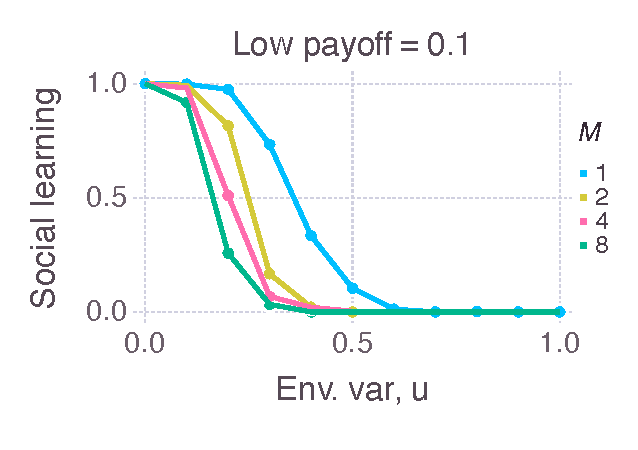
\includegraphics[width=\textwidth]{
      {Figures/SL_over_u_lowpayoff=0.1_nbehaviors=2.pdf}
    }
    \centering
    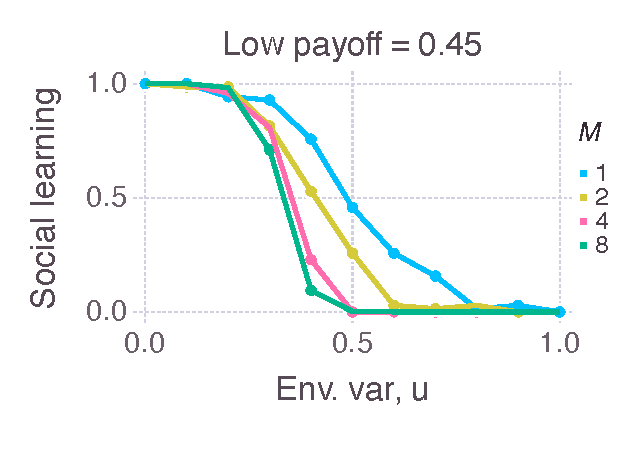
\includegraphics[width=\textwidth]{
      {Figures/SL_over_u_lowpayoff=0.45_nbehaviors=2.pdf}
    }
    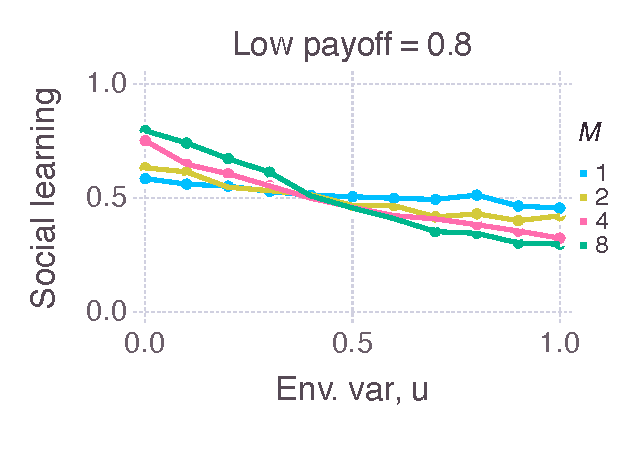
\includegraphics[width=\textwidth]{
      {Figures/SL_over_u_lowpayoff=0.8_nbehaviors=2.pdf}
    }
  \end{subfigure}%
  \begin{subfigure}[t]{0.33\textwidth}
    \centering
    \caption{$B = 4$, $M=2,4,8$}
    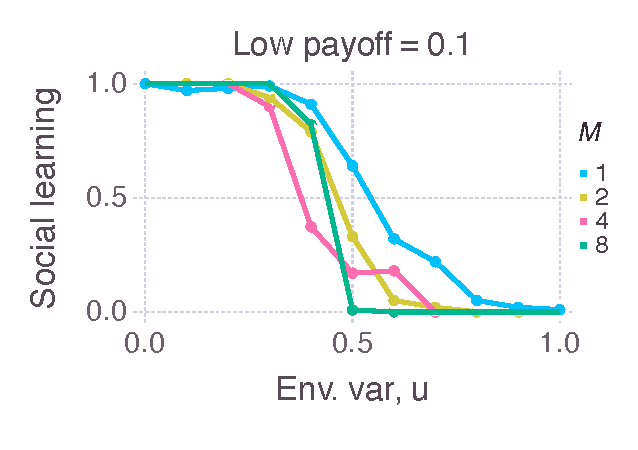
\includegraphics[width=\textwidth]{
      {Figures/SL_over_u_lowpayoff=0.1_nbehaviors=4.pdf}
    } \\
    \centering
    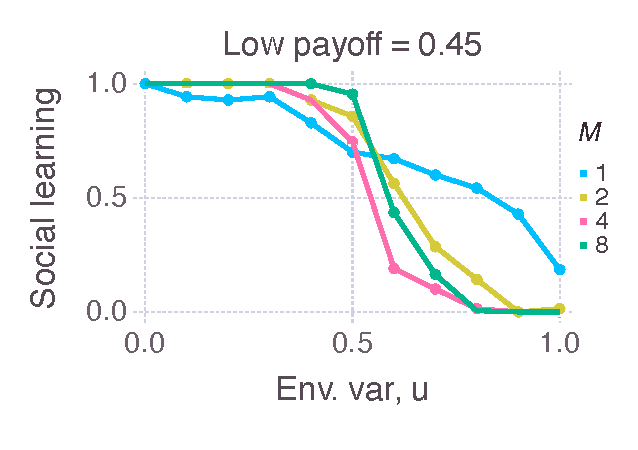
\includegraphics[width=\textwidth]{
      {Figures/SL_over_u_lowpayoff=0.45_nbehaviors=4.pdf}
    } \\
    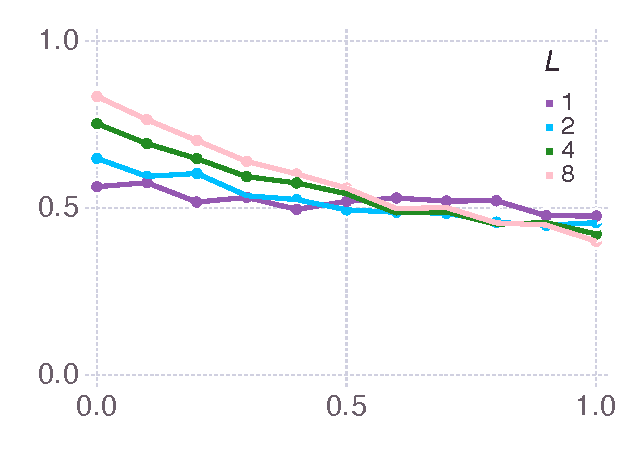
\includegraphics[width=\textwidth]{
      {Figures/SL_over_u_lowpayoff=0.8_nbehaviors=4.pdf}
    }
  \end{subfigure}
  \begin{subfigure}[t]{0.33\textwidth}
    \centering
    \caption{$B = 10$, $M=5,10,20$}
    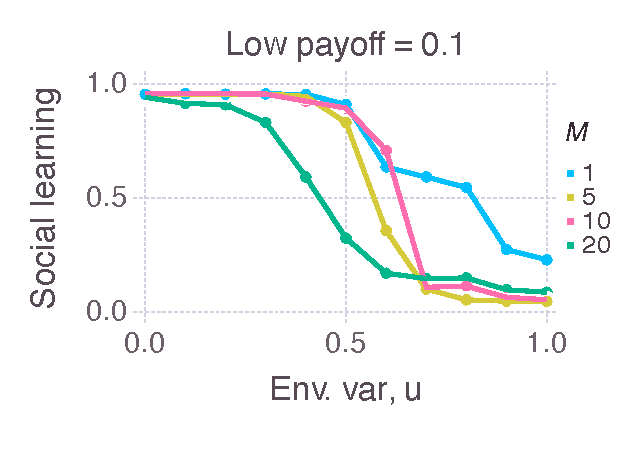
\includegraphics[width=\textwidth]{
      {Figures/SL_over_u_lowpayoff=0.1_nbehaviors=10.pdf}
    } \\
    \centering
    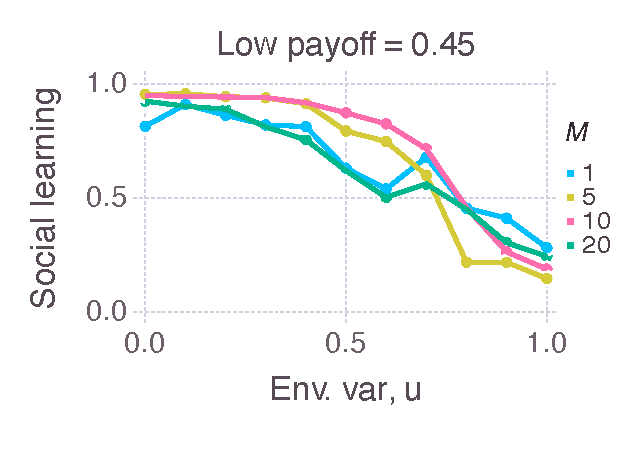
\includegraphics[width=\textwidth]{
      {Figures/SL_over_u_lowpayoff=0.45_nbehaviors=10.pdf}
    } \\
    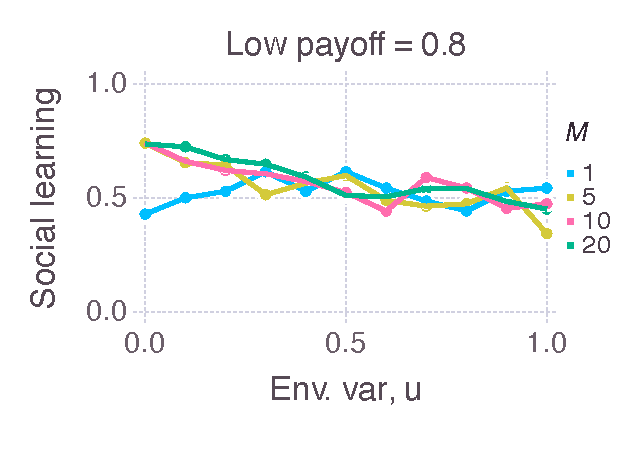
\includegraphics[width=\textwidth]{
      {Figures/SL_over_u_lowpayoff=0.8_nbehaviors=10.pdf}
    }
  \end{subfigure}
  
  
\end{figure}
